\documentclass[11pt]{amsart}
%%% WARNING: Do NOT change the page size, fonts, or margins!  Penalties will apply.


\usepackage{graphicx}
\usepackage{amssymb, amsmath, amsthm}
\usepackage{places} %enables \FloatBarrier, which prevents figures and tables from going below it.
%\usepackage{hyperref} %makes cross references into hyperlinks. 
\usepackage{amsmath, amssymb, amsthm, amsfonts, algpseudocode, algorithm, bbm, color, fixmath, float, graphicx, hyperref, listings, mathrsfs, mathtools, subfig, times}

%Needed commands
\newcommand*{\w}{\mathbf{w}}
\newcommand*{\x}{\mathbf{x}}
\newcommand*{\y}{\mathbf{y}}
\newcommand*{\z}{\mathbf{z}}
\newcommand*{\R}{\mathbb{R}}
\newcommand*{\E}{\mathbb{E}}
\newcommand*{\0}{\mathbf{0}}
\newcommand*{\minimizer}{\mathbf{x}^*}
\newcommand*{\dprime}{{\prime\prime}}
\newcommand{\li}[1]{\lstinline[prebreak=]!#1!}
\newcommand{\pseudoli}[1]{\lstinline[style=pseudo]!#1!}
\newcommand{\trp}{^{\mathsf T}} 
\newcommand{\im}{{i\mkern1mu}}
\newcommand{\Real}{\mathchardef\Re="023C}
\newcommand{\Imag}{\mathchardef\Im="023D}
\newcommand\norm[1]{\left\lVert#1\right\rVert}
\newcommand*\diff{\mathop{}\!\mathrm{d}}
\newcommand*\Eval[3]{\left.#1\right\rvert_{#2}^{#3}}

%Operators
\DeclareMathOperator{\argmin}{argmin}
\DeclareMathOperator{\argmax}{argmax}

%Link set up
\hypersetup{
    colorlinks=true, %set true if you want colored links
    linktoc=all,     %set to all if you want both sections and subsections linked
    linkcolor=blue,  %choose some color if you want links to stand out
    pdftitle={RL Notes},
    pdfpagemode=FullScreen
}

\endinput

%%% WARNING: Do NOT change the page size, fonts, or margins!  Penalties will apply.
%%% WARNING: Do NOT change the page size, fonts, or margins!  Penalties will apply.
\title{The Effect of Chemotherapy and Immunological Response on Breast Cancer Growth}
\author{Rebecca Gee, Henry Fetzer, Nephi Suyama, Joseph Humpherys, Oscar J. Escobar}
\date{October 29 2024} % or use \today

\begin{document}
\maketitle % this actually makes the title

\begin{abstract}
Place abstract here. The abstract summarizes in one paragraph the main question and conclusions draw from your investigation.
\end{abstract}

%% First Section
\section{Background/Motivation}

Mathematical oncology is field of oncology, the study of cancer, that employs math to study cancer and its behavior.
In the words of Dr. Rockne and MD Scott, ``it [serves] as a bridge between $\ldots$ the biologist, and the practicing clinician." \cite{IntroMathOnc}
One of the biggest application of mathematical modeling in oncology is tumor growth modeling.
In mathematical oncology, tumor growth modeling seeks to understand and model the characteristics and dynamics that govern general cancer growth.
Moreover, it seeks also to understand and model the relationship between cancer and the systems that fight against it as well as the response of the cancer itself to these systems.

The primary main purpose of tumor growth modeling is to first develop a general tumor growth model in the absence of any intervention.
Secondarily, it seeks to model the response to external factors such as immunological response or treatment. 
And thirdly, the modeling will then add tumor resistance and active fighting against any form of treatment be it from the immune system or other treatments.
In the absence of any intervention, several models have been made to try to show the growth of a tumor, measured by \textit{tumor burden}, denoted $T$, (see\ \ref{appendix: defs} for definitions), as a function of time $t$.
The models range from simple ODEs such as linear growth, or logistic growth, to more complicated models employing stochastic differential equations and algebraic differential equations. 
The main hope of these general growth models is to be able to use these models to develop more personable treatment to individuals facing the plight of cancer\ \cite{YinMoes}.

The more commonly used models due to their simplicity are linear, exponential, and logistic models (see\ \ref{appendix: models} for equations).
However, these do not accurately reflect the full and overall growth of observed cancers with the exception of a few cancer scenarios.
That is, they fail to generalize to the dynamics a cancer will exhibit: primarily that it has slow exponential rate and a maximal size.
In particular, the exponential model\ \eqref{eq: exp} is characterized by an infinite growth as $t$ increases which does not reflect the fact that a tumor can have a maximum size, even when considering a death rate.
Moreover, the logistic model\ \eqref{eq: logistic} converges too fast to the max size, $T_{\max}$, a tumor can be\ \cite{Steb23}.
As such, a need for a model that can firstly exhibit a slow exponential rate and then a slow convergence to the carrying capacity is preferred to others that only exhibit one of these two characteristics.

When it comes to treatment, most cancers typically use a combination for surgery, chemotherapy, and radiation therapy for treatment.
In breast cancer, surgery is the primary treatment which is not well suited for math modeling. 
Surgery removes as much as the cancer as possible so that any modeling growth would just have a sudden vertical drop in tumor burden at the time the surgery is removed causing discontinuities in the modeling.
For breast cancer, chemotherapy, be it neoadjuvent or adjuvent (see\ \ref{appendix: defs}), is the most common treatment supplement to surgery, being the primary treatment.

Most models for tumor growth in response to chemotherapy are primarily based on chemotherapy affecting cells at specific cell-cycles but mainly seeking to model the resistance of a specific tumor to the given drug or drugs.
Moreover, they also focus on the effects after one dose and not on a treatment plan that incorporates the frequency of the treatment.
Ophir Nave did describe that whenever chemotherapy is introduced into a model the drug would interact with both the immune system and cancer itself\ \cite{NAVE2022e09288}.
Moreover, it should also be some sort of summation of the dosage effects that wanes through the passage of time but may perhaps have a sudden and rapid change in the tumor growth as modeled by Nave in\ \eqref{eq: NavePersonalChemo}.

Most models employ a sort exponential decay of the administered drug to the patient to get the rapid effect that a chemotherapy drug has on the tumor burden (e.g.\ \eqref{eq:PanettaExpDec}).
These are also specific to a certain phase of the cell state, but despite their specificity, at times ignore the negative effects on the immune system.
Further, the effect the drug has on the tumor burden is usually also attributed to only the drug itself and the effects, while at times minimal, of the immune system fighting the cancer is omitted.
Given these characteristics, it is of interest to find an expression for the effect of chemotherapy that has a rapid change in tumor burden and either on all cells or at specific cell-states but also has an effect on the immune system.

On the other hand, the immune system naturally patrols the body in search of foreign bodies to kill and prevent diseases.

This patrolling involves not just for foreign bacteria but also abnormal cells such as cancer cells. 
The modeling for tumor-immunological response typically look at relationship between natural killer cells (NK) and cytotoxic T-cells (CD8+)$^+$ (see\ \ref{appendix: defs}) and how they affect tumor growth. The NK cells are Although there are many other cells which contribute to an immune response, NK cells and CD8 cells are the only ones which directly kill the cancer cells in breast cancers \cite{Amens21}. The CD8+ cells are recruited to kill the cancer by the NK cells, and from this interaction arises a relation between the populations of the NK, CD8+, and cancer cells. 
Unfortunately, many of the models which examine the relationship between cancer and the immune system do not include analysis of the interactions which occur once chemotherapy has begun. Because of the immunocomprimising effects of radiation and chemotherapy, the body's ability to fight tumors naturally will decrease, leading to interesting dynamics of the cell populations.

The patrolling and immediate responses are given by the innate immune system and helper response to anything missed by the immediate response as well as targeted response is handled primarily by the adaptive immune system (see\ \ref{appendix: defs}).
Majority of models, like those in\ \ref{eq: dePillisTumorImmuno} or\ \ref{eq: AlharbiTumorImmuno}, look at these two parts of the immune system as  a whole and its interaction with the tumor and normal cells.
That is, they do not look at the specific immune cells interacting with the cancer other than the collective response of the immune system on tumor growth.
But as mentioned by de Pillis et. al, ``in some applications, it is not sufficient to represent the immune response with a single homogeneous population of
effector killer cells\ \cite{dePillis2014461}."


TODO Add graph showing the different models

Thus, our focus is to model the growth of a HER2 positive breast cancer in relation to immunological system response of the Nk and CB cells and under neoadjuvent (see \ref{appendix: defs}) chemotheraphy.

%\begin{figure}[htb]
%\begin{center} %Put your images in a figure like this
%\includegraphics[width=\textwidth]{Myfig.pdf} % Better to make them pdfs than png or gif or jpeg
%\end{center}
%\caption{Plots should be high resolution (pdf 300dpi), uncluttered, a reasonable size, and easily readable and understandable.  All figures should have a complete caption that helps the reader make sense of the figure even if they haven't read the paper yet. Here is an example: This figure shows the risk or mean squared error (in black) of for a generic family of regression models as a function of model complexity (the number of free parameters in the model).  The generalized aliasing decomposition shows that the risk is the sum of three parts: Model insufficiency (red), Data insufficiency (green), and Aliasing (blue).  Model insufficiency is monotonically decreasing as a function of complexity, Data insufficiency vanishes when the number of parameters is less than the number of training points (the classical regime), but increases monotonically in the modern regime (where the number of parameters is greater than the number of data points).  Aliasing generally increases up to the interpolation threshold and decreases thereafter, converging to zero almost surely as the number of parameters goes to infinity.  
%}
%\label{fig:MeanSquaredError} % for automatic cross referencing
%\end{figure}



%% Second Section 
\section{Modeling}

%% Finite Difference methods, feel free to edit or place where you would like --Rebecca
In solving the original Gompertz model, finite difference methods were used because of their simplicity yet relative accuracy. The local truncation error for Forward Euler can be found as follows $\tau_i = |T^\prime(t_i) - \frac{T(t_i + h) - T(t_i)}{h}|$  where $T(t_i)$ is the actual solution at time $i$. Using Taylor Series, we can expand this to $\Bigl |T^\prime(t_i) - \frac{T(t_i) + hT^\prime(t_i) + h^2T^\dprime(t_i) + h^3T^{\prime\prime\prime}(t_i) + O(h^4) - T(t_i)}{h}\Bigr |$ which simplifies to $|-hT^\dprime(t_i) - h^2T^{\prime \prime \prime}(t_i) + O(h^3)| = O(h)$. So although quick to code and compute, there is a relatively large error term. 
%% End Finite Difference methods

The \textit{Gompertz} model is a logistic model that was created to describe the growth of human mortality in 1825 by Benjamin Gompertz.
In particular, the ODE is given by
\begin{equation}
	\frac{\diff T(t)}{\diff t} = k_g T \ln \biggl(\frac{T_{\max}}{T} \biggr) \label{eq: gompertz},
\end{equation}
where $k_g$ is a growth constant of the tumor, $T$ is the total number of cancer cells, and $t$ is days.
The solution to the ODE is of sigmoidal nature.
Like the logistic growth model \eqref{eq: logistic}, the Gompertz model starts off with a quasi-exponential growth at the beginning that is short lived.
However, unlike the logistic model, the Gompertz model slowly converges to the carrying capacity of that a tumor can have with available nutrients.
That is, the Gompertz model slows its growth first and more significantly than a logistic model while still converging, slowly, towards the carrying capacity \cite{Steb23} .
Getting the derivative of \eqref{eq: gompertz} and setting it equal to 0, gives us that  the inflection point of the Gompertz model is at $\frac{T_{\max}}{e}$.
This is the point when 36.8\% of the carrying capacity has been reached compared to the inflection point of the logistic model that occurs at half the carrying capacity.
Given these characteristics, the Gompertz model is a popular and good choice for modeling tumor growth.

For chemotherapy effects, seeing that models are derived as exponential decays of the drug-dose and are dependent on the type of the type of drug administered as well as the percentage of cancer killed at a specific cell-state, we opted to work with the model proposed by Bethge et al (which is similar to the one given by de Pillis and Radunskaya \eqref{eq: Pillis}). The chemotherapy differential expression is 
\begin{equation}
	f \mu c(t) T, c(t) = e^{-\gamma t} \label{eq: chemo},
\end{equation}
where $\mu$ represents the drug sensitivity of cells (thereby implying drug effectiveness), $c(t)$ is the concentration of the given drug with a rate modeled by a decay constant $\gamma=\frac{\ln{2}}{t_{1/2}}$ after the half-life of the drug, and $f$ is is the proportion of cells that are in specific cell-cycle such that chemotherapy affects those cells specifically.
If the given drug affects all cells equally irrespective of cell cycle, then $f$ is equal to 1.

The chemotherapy differential expression specifically models the rate of change in respect to time of the death or removal of tumor cells by the given drug.
At $t=0$, we would expect a high number of cells to be killed off, and as time continues, we would expect to see that the effectiveness of the drug levels off (hence the decay).
Moreover, depending on how good or strong the drug is, we would expect to have a different rate of change which is the purpose of the half life in $\gamma$ and the $f$ constant.
Adding \eqref{eq: chemo} to our growth in \eqref{eq: gompertz} gives 
\begin{equation}
	\frac{\diff T(t)}{\diff t} = k_g T \ln \biggl(\frac{T_{\max}}{T} \biggr) - f \mu c(t) =k_g T \ln \biggl(\frac{T_{\max}}{T} \biggr) - f \mu e^{-\gamma t} \label{eq: gompertz-chemo}.
\end{equation}
For our purposes, we chose to go with a chemotherapy treatment plan of one dose every two weeks for a total of 14 doses. 



The combination of the two models requires some thought. The Gompertz-Chemo integrated model for tumor burden can be added in place of the logistic growth factor in the immune system model, but the effects of the chemotherapy on the immune cells cannot be ignored. Although sources were inconclusive on whether the chemotherapy directly killed the NK and CD8+ cells, it is known that all cells are negatively affected by the therapy. We make the assumption that the number of NK and CD8+ cells affected by the chemotherapy is proportional to \eqref{eq: chemo} and the number of NK and CD8+ cells. This results in the following system of equations.

\begin{equation} \label{eq1}
\frac{dT}{dt} = aT(1-bT) - cNT - D 
\end{equation}
\begin{equation} \label{eq2}
\frac{dN}{dt} = \sigma - fN +\frac{gT^2}{h + T^2}N - pNT - Nf \mu e^{-\gamma t}
\end{equation}
\begin{equation} \label{eq3}
\frac{dL}{dt} = - mL +\frac{jD^2}{k + D^2}L - qLT + rNT
\end{equation}
\begin{equation} \label{eq4}
D = d\frac{(L/T)^\lambda}{s + (L/T)^\lambda}T
\end{equation}



 The primary aspect of the project is the modeling of the chosen phenomenon. If your group's repeated attempts resulted in abject failure, or your group succeeded, detail them in this section. Be sure to account for the various attempted models and why they were not appropriate. Include numerical simulations for each attempted model.  Reference figures and plots, like Figure~\ref{fig:MeanSquaredError}.


%% Third Section
\section{Results}

\begin{figure}[htb]
\begin{center} %Put your images in a figure like this
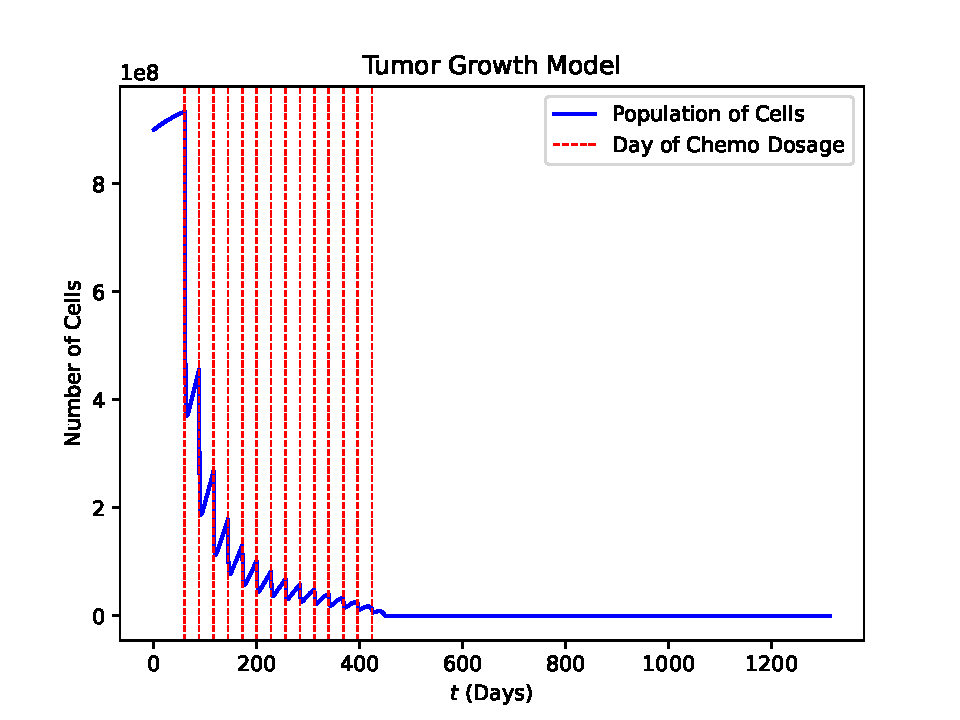
\includegraphics[width=\textwidth]{./images/image.pdf} % Better to make them pdfs than png or gif or jpeg
\end{center}
\caption{The growth of breast cancer growth as modeled by
}
\label{fig:MeanSquaredError} % for automatic cross referencing
\end{figure}



Clearly and succinctly state and describe the conclusions that you can draw from the model you have achieved (or the many failed attempts). Does your model(s) perform well quantitatively or qualitatively?

%%Fourth Section
\section{Analysis/Conclusions}

Discuss the appropriateness of the techniques/methods you employed in modeling. Did your group appropriately model the chosen phenomenon? If not, what different steps could you have taken if you had more time? What did you learn about the techniques/method that were used in the group project? If your model was successful, what additional insight/conclusions could you obtain from it? For instance, if you had a successfully modified SIR model, how might it affect different government policy? If you had a successful model for the spread of inaccurate information on social media, how might it be implemented to help reduce the spread of inaccurate information?



This part should all be done before you get to \emph{page 11}.  The bibliography can spill on to page 11, but we won't read text that goes past page 10.

\appendix
\section{Definitions}
\label{appendix: defs}
The following definitions are derived from the National Cancer Institute, unless otherwise stated
\begin{itemize}
	\item Adaptive Immune System: the part of the immune system that specifically targets the germs or foreign substances that are causing an infection. In order to do this, this system needs to first recognize the substance as such. Therefore, this system is slower and needs training. CB8$^+$ cells are part of this system.
	\item Cancer:  a term for diseases in which abnormal cells divide without control and can invade nearby tissues
	\item Chemotherapy: a cancer treatment where drugs are used to kill cancer cells or stop them from dividing
		\begin{itemize}
			\item Neoadjuvent Chemotherapy: chemotherapy administered before the primary treatment of the tumor is performed. Typically, surgery is the primary treatment. Its main goal is to shrink the tumor so that it is easier to remove.
			\item Adjuvent Chemotherapy: Chemotherapy administered after primary tumor treatment is administered. Its intent is to lower the risk of the cancer returning.
		\end{itemize}
	\item Cytotoxic/CB8$^+$ T-cell: is a T-lymphocyte that kills or infected cells or cells that are damaged in other ways. They are not natural killers and as such have to be trained to kill cancer. (Mayo clinic)
	\item Innate Immune System: the part of the immune system that is the first line of defense against intruders or unknown foreign cells in the body. It responds to all foreign substances in the same manner (National Library of Medicine). It can be thought of as "kill first, ask questions later." NK cells are part of this system.
	\item Log-kill Hypothesis: when growth of a cancer is exponential—increasing by a constant fraction of itself every fıxed unit of time—then in the presence of effecive anticancer drugs it also shrinks by a constant fraction \cite{LogKill}
of itself
	\item Tumor: an abnormal mass of tissue that forms when cells grow and divide more than they should or do not die when they should. Tumors may be \textit{benign} (not cancer) or \textit{malignant} (cancer). For this project, defined the tumor burden as the number of cancer cells in the body.
	\item Tumor burden: the size of a tumor or number cancer cells. This is the total amount of cancer found in the body.
        \item Natural Killer Cell (NK Cell): A type of immune cell that has granules (small particles) with enzymes that can kill tumor cells or cells infected with a virus. A natural killer cell is a type of white blood cel
\end{itemize}

\section{Models}
\label{appendix: models}
\begin{itemize}

	\item Tumor Growth Models:
		\begin{itemize}
	\item Linear growth: 
		\begin{equation}
			\frac{\diff T}{\diff t} = k,
			\label{eq: lin}
		\end{equation} 
		where $k$ is the growth rate
	\item Exponential Growth:
		\begin{equation}
			\frac{\diff T}{\diff t} = kT \label{eq: exp}
		\end{equation} 
	 or with a death rate constant of $d$, $\frac{\diff T}{\diff t} = (k-d)T$
	\item Logistic Growth: 
		\begin{equation} 
			\frac{\diff T}{\diff t} = kT \biggl(1- \frac{T}{T_{\max}}\biggr)\label{eq: logistic},
		\end{equation}
		where $T_{\max}$ is the max size a tumor can be, which is equivalent to the carrying capacity.
		\end{itemize}
		
	\item Chemotherapy Models: 
		\begin{itemize}
			\item Exponential Decay: Pillis and Radunskaya modeled the mix of immunotherapy and chemotherapy on tumor growth. In particular, they modeled the drug as an exponential decay given by 
				\begin{equation}
					G_M = -\gamma M \label{eq: Pillis},
				\end{equation}
				where $M=M(t)$ is the concentration of the drug in the bloodstream at some time $t$.
				
			\item Panetta also used an exponential but considering the frequency between doses as
				\begin{equation}
					g(t) = h e^{-\gamma(t-n-\tau)} \label{eq:PanettaExpDec},
				\end{equation}
				where $g(t)$ is the effects of the chemotherapy drug, $\gamma$ is the decay of the drug, $n$ is number of doses, and $\tau$ is the period between doses.
				
			\item Personalized treatment: Ophir Nave modeled a personalizable treatment plan as 
				\begin{equation}
					\mathscr{F} = \sum_{k=0}^n q(t-mk) \mathscr{H} (t-mk)e^{\frac{t-mk}{0.5}}\label{eq: NavePersonalChemo},
				\end{equation}
				where $n$ is the duration of the treatment, $m$ is the interval between treatments, and $\mathscr{H}$ a unit step function.
		\end{itemize}
	\item Immunological Response Models:
		\begin{itemize}
			\item Alharbi \& Sham Rambely: their modeling equations looked at the interaction of tumor cells and the immune system, $I$, as a whole as well as normal cells , $N$, (non-immune, non-tumor cells). They described the relationships by (using a logistic growth for tumor $T$):
				\begin{eqnarray}
					\begin{aligned}
						\frac{\diff N}{\diff t} &= rN(1-\beta_1 N) - \eta NI - \gamma NT \\
						\frac{\diff T}{\diff t} &= \alpha_1T(1-\alpha_2T) + \beta_2 NT - \alpha_3 T1 \\
						\frac{\diff I}{\diff t} &= \sigma - \delta I _ \frac{\rho N I}{m+N} + \frac{\rho_1 TI}{m_1 + T} - \mu NI - \mu_1 TI \label{eq: AlharbiTumorImmuno}
					\end{aligned}
				\end{eqnarray}
			\item dePillis et. al: they modeled the primary interaction between effector cells, $E$, like CB8$^+$, and the tumor, $T$ by using logistic growth and 
				\begin{eqnarray}
					\begin{aligned}
						\frac{\diff T}{\diff t} &= a_1T(1-b_1T) - c_2ET - c_3NT - k_2(1-e^{-u}) \\
						\frac{\diff N}{\diff t} &= a_2(1-b-2N) - c_4NT - k_3 (1-e^{-u})\label{eq: dePillisTumorImmuno}
					\end{aligned}
				\end{eqnarray}
		\end{itemize}
	\item Growth-Chemo-Immune PDE System: Ansarizadeh, Singh, and Richards modeled tumor cells using a system of PDEs. Specifically, they used a logistic model for the normal cells $N$, tumor $T$, immune $I$, and the chemotherapeutic drug $U$. For them, the drug was only active for certain phases of the cell division cycle the expression $1-e^{-U}$ was used to denote the fraction of cells killed.
		\begin{eqnarray}
			\begin{aligned}
				\frac{\partial N}{\partial t} &= r_2 N (1-b_2)N - c_4TN - a_3(1-e^U)N + D_N \frac{\partial^2 N }{\partial x^2} \\
				\frac{\partial T}{\partial t} &= r_1 N (1-b_1 T) - c_2 IT - c_3TN - a_2(1-e^{-U})T + D_T \frac{\partial^2 T }{\partial x^2} \\
				\frac{\partial I}{\partial t} &= s + \frac{\rho IT}{\alpha + T} - c_1 IT - d_1 I - a_1(1-e^{-U})I +D_I \frac{\partial^2 I }{\partial x^2} \\
				\frac{\partial U}{\partial t} &= v(t) -d_2U + D_U \frac{\partial^2 U}{\partial x^2}\label{eq:GrowthChemoImmunoPDE}
			\end{aligned}
		\end{eqnarray}
\end{itemize}


%%%%%%%%%%%%%%%%%%%%%%%%%%%%%%%%%%%%%
%% Bibliography below
%%%%%%%%%%%%%%%%%%%%%%%%%%%%%%%%%%%%%
%\FloatBarrier % Keep the figures from being put after the bibliography
\newpage
%% If using bibtex, leave this uncommented
\bibliography{refs.bib} %if using bibtex, call your bibtex file refs.bib
\bibliographystyle{alpha}
%% If not using bibtex, comment out the previous two lines and uncomment those below
%\begin{thebibliography}{99}
%\bibitem{Vandermeersch} First reference goes here
%\end{thebibliography}

\end{document}
